\begin{frame}
\frametitle{B+ деревья}
\begin{itemize}
  \item B+ дерево - идеально сбалансированное сильно ветвистое дерево
  поиска, которое хранит значения только в листьях:
  \begin{itemize}
    \item растояние от корня до всех листьев одинаковое;
    \item каждый узел кроме корня хранит не менее B ключей, где B
    некоторый фиксированный параметр дерева;
    \item словарь хранит пары - (ключ, значение) - все внутренние узлы
    хранят только ключи, и только листья хранят полные пары.
  \end{itemize}
\end{itemize}
\end{frame}

\begin{frame}
\frametitle{Реализации B+ деревьев}
\begin{itemize}
  \item Есть много подходов к реализации B+ деревьев и, соответсвенно, к
  балансировке
  \begin{itemize}
    \item мы рассмотрим классический вариант B+ деревьев с балансировкой
    снизу вверх;
    \item а также то, что называется COW B+ деревья - это самый простой
    вариант;
    \item COW B+ деревья реально используются на практике в ФС Btrfs.
  \end{itemize}
\end{itemize}
\end{frame}

\begin{frame}
\frametitle{Узел B+ дерева}
\begin{center}
  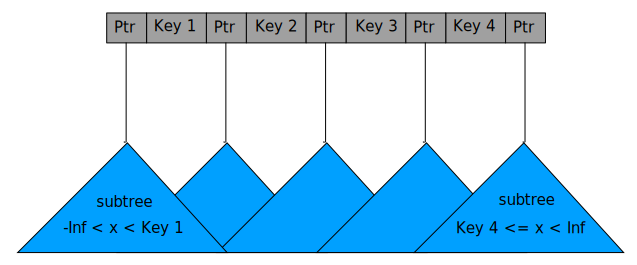
\includegraphics[width=.6\linewidth]{bnode.png}
\end{center}
\begin{itemize}
  \item Каждый узел хранит от $B$ до $2B$ ключей и ссылок на следущие узлы:
  \begin{itemize}
    \item корень - исключение, он может хранить произвольное количество
    ключей и ссылок на следующие узлы;
    \item листья не хранят ссылки на следующие узлы;
    \item ограничение весьма условно, не редко границы делают шире: $B$ и
    $4B$, чтобы обеспечить гистерезис.
  \end{itemize}
\end{itemize}
\end{frame}

\begin{frame}
\frametitle{Поиск в B+ дереве}
\begin{itemize}
  \item Поиск в B+ дереве похож на поиск в бинарном дереве поиска:
  \begin{itemize}
    \item что не удивительно, ведь B+ дерево тоже является деревом поиска;
    \item на каждом шаге просто выбираем поддерево, в котором может
    содержаться нужный ключ и повторяем поиск рекурсивно, пока не дойдем до
    листа.
  \end{itemize}
  \item Сложность поиска:
  \begin{itemize}
    \item для нас в первую очередь важны операции обращения к диску - чтения
    и записи узлов дерева;
    \item количество чтений - высота дерева;
    \item все узлы кроме, возможно, корня, содержат как миниум $B$ ключей;
    \item высота дерева ограничена снизу как $1 + log_B N$, где $N$ -
    количество пар в дереве.
  \end{itemize}
\end{itemize}
\end{frame}

\begin{frame}
\frametitle{Вставка в B+ дерево}
\begin{itemize}
  \item Вставка в целом протекает так же как и поиск:
  \begin{itemize}
    \item на каждом шаге мы выбираем поддерево, в которой должен попасть
    новый ключ;
    \item но вставка может изменить количество ключей, а значит может
    нарушить ограничения на количество ключей в узле дерева - и нам придется
    это исправлять.
  \end{itemize}
  \item Допустим мы нашли нужный лист, у нас может быть два варианта:
  \begin{itemize}
    \item в листе достаточно места для нового ключа - перебалансировка не
    потребуется требуется;
    \item в листе не достаточно места - нам нужно разбить узел на два и
    поделить все ключи, включая новый, между двумя новыми узлами поровну.
  \end{itemize}
\end{itemize}
\end{frame}

\begin{frame}
\frametitle{Вставка в B+ дерево}
\begin{itemize}
  \item Если нам пришлось разбить лист на два новых узла, то нам нужно
  обновить родителя, здесь возможны несколько враинтов:
  \begin{itemize}
    \item родителя нет, а лист так же является корнем - в этом случае нужно
    создать новый пустой узел и добавить в него ссылки на два созданных узла,
    он станет новым корнем дерева;
    \item родитель сам полон и в него уже нельзя добавить ключ - в этом
    случае мы можем разбить родителя на два узла, как мы делали это с листом
    и повторить операцию рекурсивно;
    \item в родителе достаточно места для нового ключа - перебалансировка не
    требуется.
  \end{itemize}
\end{itemize}
\end{frame}

\begin{frame}
\frametitle{Удаление из B+ дерева}
\begin{itemize}
  \item Как и со вставкой для начала найдем нужный лист и нужный ключ в
  листе, далее возможны два варианта:
  \begin{itemize}
    \item в узле даже после удаление достаточно ключей - перебалансировка
    не требуется;
    \item после удаления в кзле слишком мало ключей - потребуется
    перебалансировка, возможно.
  \end{itemize}
\end{itemize}
\end{frame}

\begin{frame}
\frametitle{Удаление из B+ дерева}
\begin{itemize}
  \item Итак в узле слишком мало ключей, у нас есть несколько возможностей:
  \begin{itemize}
    \item у узла есть левый/правый брат:
    \begin{itemize}
      \item суммарно в узле и его брате достаточно ключей на два узла, то
      их можно перераспределить и обновить ключи в родительском узле;
      \item суммарно в узле и его брате не достаточно ключей на два узла,
      тогда их нужно их объединить, при этом из родителя придется удалить
      один ключ;
    \end{itemize}
    \item у узла нет братьев, а значит наш узел - корень дерева, и тут
    возможны варианты:
    \begin{itemize}
      \item в корне осталась только одна ссылка на дочерний узел - мы можем
      просто удалить этот корень и заменить его ребенком;
      \item в корне осталось больше одной ссылки - никаких модификаций не
      требуется.
    \end{itemize}
  \end{itemize}
\end{itemize}
\end{frame}

\begin{frame}
\frametitle{COW B+ дерево}
\begin{itemize}
  \item В рассмотренном ранее варианте мы сначала искали нужный лист для
  вставки/удаления, а затем двигаясь от листьев к корню восстанавливали
  инварианты дерева
  \begin{itemize}
    \item но можно во время поиска нужного листа сразу исправлять дерево
    так, чтобы инварианты не нарушались при вставке/удалениию.
  \end{itemize}
  \item Вставка:
  \begin{itemize}
    \item если при поиске нужного листа мы натыкаемся на полный узел,
    вставка в который, приведет к разбиению, то мы разбиваем его заранее
    по мере прохода вниз по дереву.
  \end{itemize}
  \item Удаление:
  \begin{itemize}
    \item аналогично вставке, но теперь мы перебалансируем если находим
    узел с малым числом ключей, при этом требуется особенная забота о
    корне.
  \end{itemize}
\end{itemize}
\end{frame}
